\section{ResNet}
ResNet的核心就是对每一个残差块,将输入与卷积后的输出相加后再传递激活函数,
而并非只将输出传递给激活函数,从而解决了模型较深时梯度消失的问题。
残差块的典型结构如图\ref{fig:ResNetArchitecture}所示。

\begin{figure}[H]
    \begin{subfigure}[c]{0.45\textwidth}
        \centering
        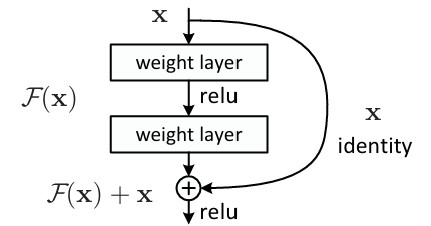
\includegraphics[width=0.8\textwidth]{./figures/ResNetArchitecture.jpg}
        \caption{ResNet残差块结构}
        \label{fig:ResNetArchitecture}
    \end{subfigure}
    \hfill
    \begin{subfigure}[c]{0.45\textwidth}
        \centering
        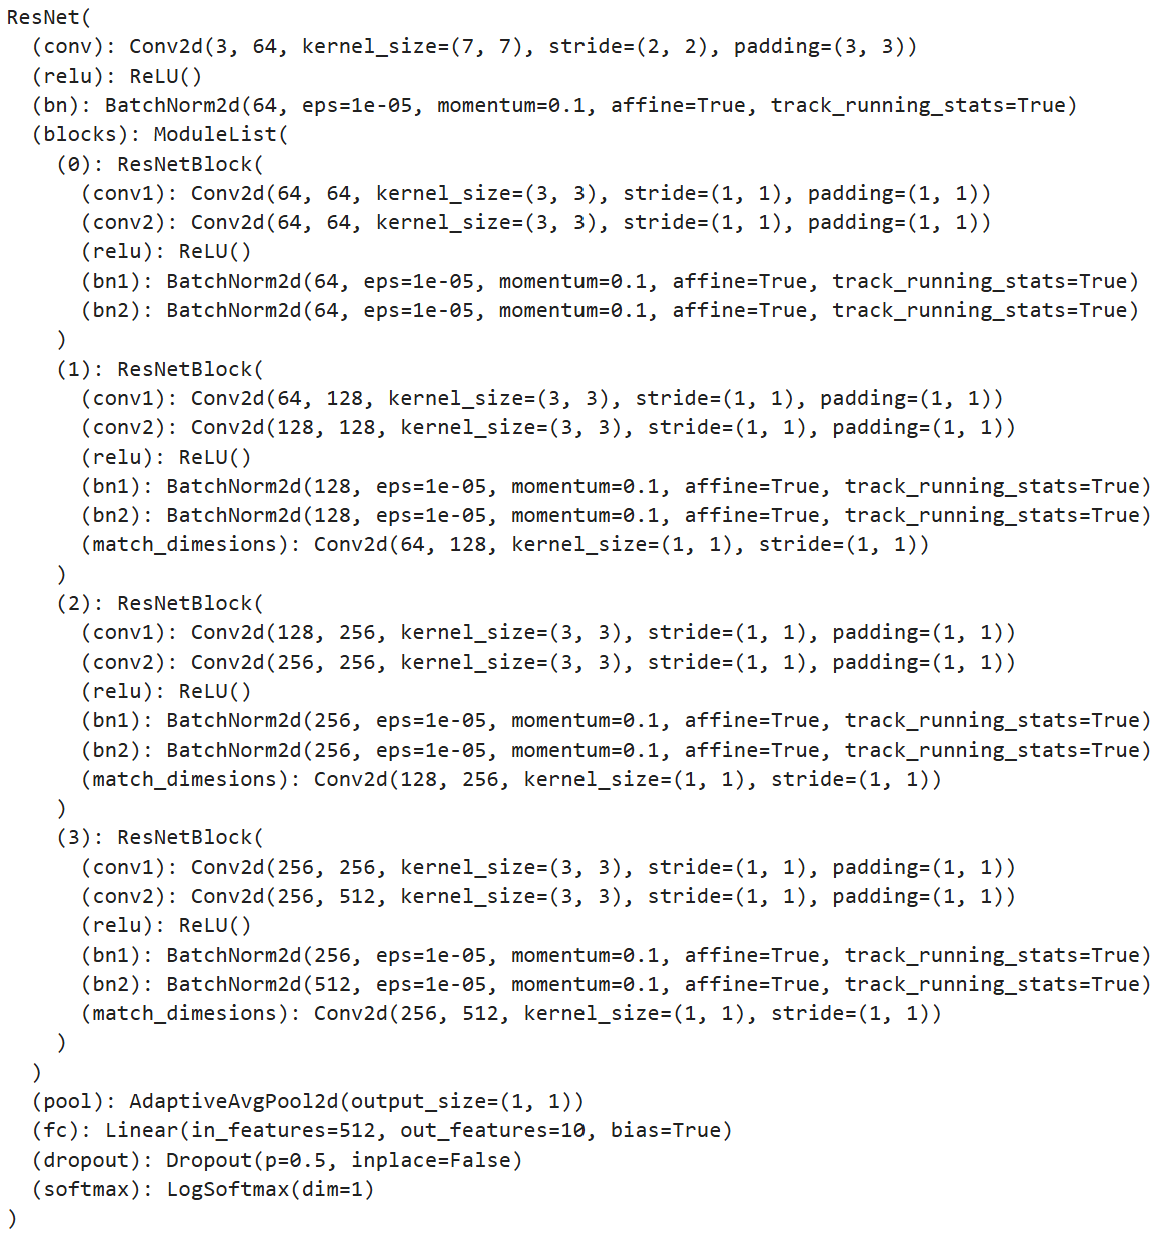
\includegraphics[width=0.8\textwidth]{./figures/MyResNet.png}
        \caption{实验采用的ResNet结构}
        \label{fig:MyResNet}
    \end{subfigure}
    \caption{模型结构}
    \label{fig:Architectures}
\end{figure}

本次实验的ResNet结构如图\ref{fig:MyResNet}所示。
每一个残差块当中都会根据输入和输出的尺寸进行判断。
如果输入和输出的尺寸不同,残差块当中会添加一个额外的卷积层,其卷积核大小为1。
输入通过该卷积层后与输出尺寸相同,从而能够完成相加操作。

实验利用CIFAR-10数据集来训练模型,损失曲线如图\ref{fig:resnetlosshistory}所示,
训练过程当中,模型在训练集上和测试集上的准确率曲线如图\ref{fig:resnetmetrics}所示。

\begin{figure}[H]
    \begin{subfigure}[c]{0.45\textwidth}
        \centering
        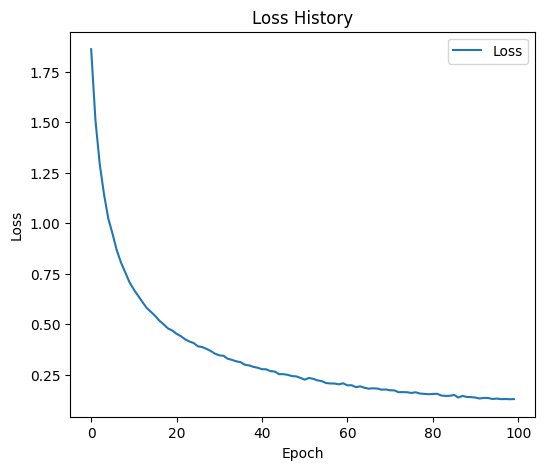
\includegraphics[width=\textwidth]{../output/resnet/loss_history.png}
        \caption{损失曲线}
        \label{fig:resnetlosshistory}
    \end{subfigure}
    \hfill
    \begin{subfigure}[c]{0.45\textwidth}
        \centering
        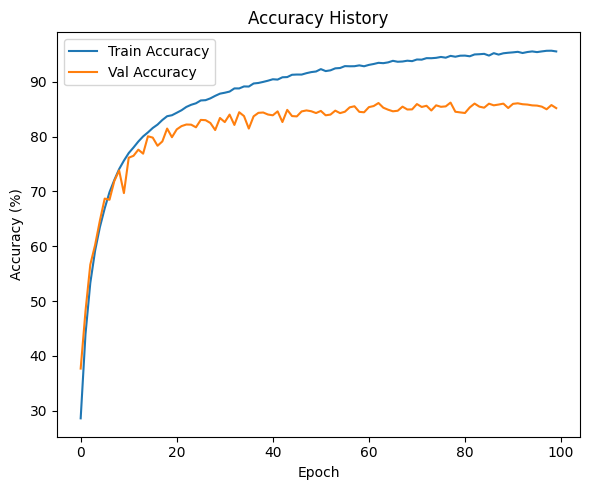
\includegraphics[width=\textwidth]{../output/resnet/metrics.png}
        \caption{准确率曲线}
        \label{fig:resnetmetrics}
    \end{subfigure}
\end{figure}

最后将模型第一个卷积层可视化。

\begin{figure}[H]
    \centering
    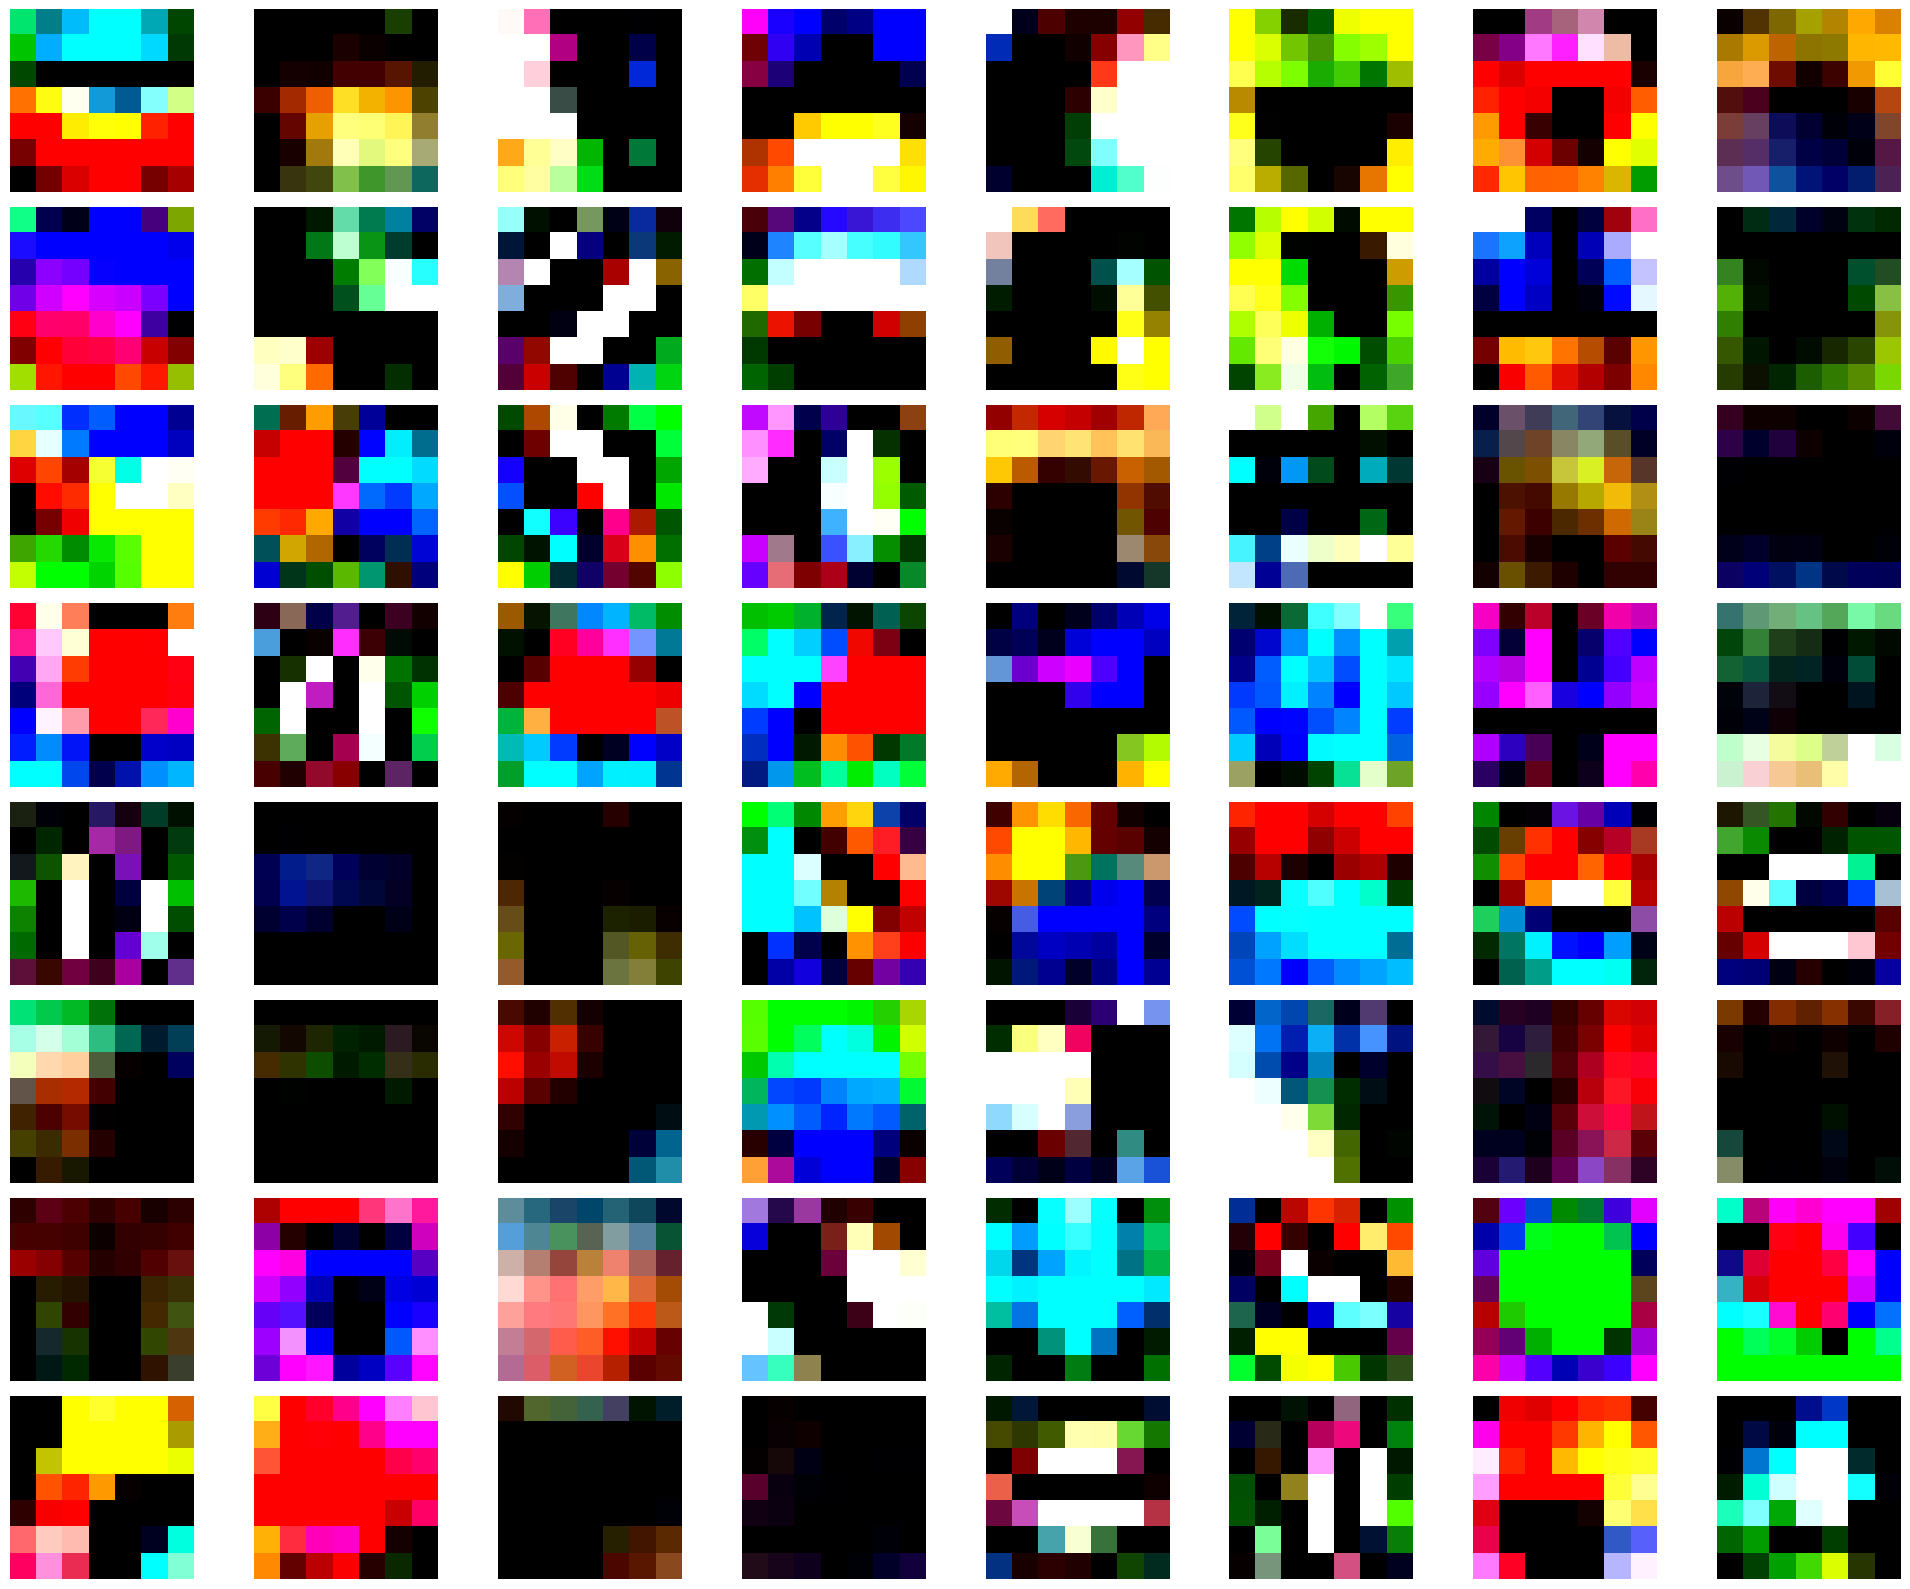
\includegraphics[width=0.5\textwidth]{../output/resnet/conv1.png}
    \caption{模型第一个卷积层}
\end{figure}